\documentclass[conference]{IEEEtran}
\IEEEoverridecommandlockouts

\usepackage{cite}
\usepackage{amsmath,amssymb,amsfonts}
\usepackage{graphicx}
\usepackage{booktabs}
\usepackage{multirow}
\usepackage{textcomp}
\usepackage{xcolor}
\usepackage{url}

\begin{document}

\title{Swarm Intelligence for Feature Selection in Disease Prediction}

\author{
\IEEEauthorblockN{Shashank Kushwaha}
\IEEEauthorblockA{Department of Computer Science and Engineering (AIML)\\
IILM University, Greater Noida, India}
\and
\IEEEauthorblockN{Anshika Srivastava}
\IEEEauthorblockA{Department of Computer Science and Engineering (AIML)\\
IILM University, Greater Noida, India}
\and
\IEEEauthorblockN{Muskan Mishra}
\IEEEauthorblockA{Department of Computer Science and Engineering (AIML)\\
IILM University, Greater Noida, India}
\and
\IEEEauthorblockN{Roushan Kumar}
\IEEEauthorblockA{Department of Computer Science and Engineering (AIML)\\
IILM University, Greater Noida, India}
\and
\IEEEauthorblockN{Niharika Chaudhary}
\IEEEauthorblockA{Assistant Professor\\
IILM University, Greater Noida, India}
}

\maketitle

% ---------------------------------------------------------------------------
\begin{abstract}
Feature selection is an important stage in machine learning-based disease
prediction because irrelevant or redundant input variables increase
computational cost and complicate model interpretation. This paper applies
Binary Particle Swarm Optimization (BPSO) to select compact feature subsets
for binary disease classification. Each particle represents a candidate
feature subset, and the fitness function balances inner cross-validated
accuracy against subset size. BPSO is evaluated on five public benchmarks
(breast cancer, chronic kidney disease, heart disease, liver disease and
diabetes) and compared with nine alternatives---all features, a binary genetic
algorithm, mutual-information and ANOVA-F filters, recursive feature
elimination, L1-regularised logistic regression and random subsets---using
five classifiers and $5\times$ repeated stratified 10-fold cross-validation,
with all selection and tuning performed inside the training folds. BPSO
removed 38--58\,\% of the features on every dataset while keeping the F1-score
within about 0.015 of the all-feature model, and it was significantly better
than random subsets of equal size on two datasets. However, across 25
dataset--classifier settings it did not outperform simpler methods: its
average Friedman rank was 7.20 of 10 (Friedman $\chi^2=76.7$, $p<10^{-12}$),
comparable to the genetic algorithm (7.28) and behind all features (3.68) and
cross-validated filters (3.80--3.88). On these low-dimensional clinical
datasets the main benefit of BPSO is a smaller model, not higher accuracy.
\end{abstract}

\begin{IEEEkeywords}
Swarm intelligence, feature selection, disease prediction, Binary Particle
Swarm Optimization, machine learning, classification.
\end{IEEEkeywords}

% ---------------------------------------------------------------------------
\section{Introduction}

Machine learning is increasingly studied for analyzing medical data and
supporting disease-risk prediction. A dataset may contain multiple clinical
variables, but not every variable contributes equally to prediction.
Irrelevant or redundant features may increase training time, make models
harder to interpret, and potentially reduce generalization. In clinical
settings, the cost of collecting each variable is also a practical concern,
since every additional measurement may require a test, time, and resources
from the patient and the healthcare provider.

Feature selection aims to identify a useful subset of the available variables
while retaining predictive information. Swarm intelligence algorithms are
population-based optimization methods inspired by collective behavior in
nature, such as the movement of bird flocks and fish schools. Particle Swarm
Optimization (PSO) is one such method. Its binary variant, Binary Particle
Swarm Optimization (BPSO), represents feature selection as a search over
binary vectors, where each bit indicates whether a particular feature is
included in the model.

This paper evaluates a BPSO-based feature-selection workflow for disease
prediction on five public datasets. The approach is compared against models
trained with all available features and against eight alternative
feature-selection methods, under a protocol in which feature selection,
preprocessing and hyperparameter tuning never see the test data. The aim is
to determine whether a compact subset of features can support prediction with
acceptable loss of performance, and to describe each stage explicitly so that
the experiment can be reproduced. The contributions are:
\begin{itemize}
\item a BPSO wrapper with a size-penalised fitness function, fitness caching
and an empty-subset repair rule;
\item a leakage-free nested evaluation over five datasets, ten
feature-selection strategies and five classifiers (12\,500 outer-fold
evaluations);
\item paired significance tests, a Friedman/Nemenyi ranking, stability,
runtime and sensitivity analyses;
\item open-source code, results and an online demonstration.
\end{itemize}

% ---------------------------------------------------------------------------
\section{Problem Statement}

Given a labelled medical dataset with $d$ input features, the goal is to
select a subset of features that balances predictive performance and subset
compactness. Let the feature vector be
\begin{equation}
X = \{x_1, x_2, \ldots, x_d\}.
\end{equation}
A binary selection vector is defined as
\begin{equation}
z = [z_1, z_2, \ldots, z_d], \quad z_j \in \{0,1\},
\end{equation}
where $z_j = 1$ means feature $j$ is selected and $z_j = 0$ means it is
excluded. The selected subset is
\begin{equation}
X_z = \{x_j \mid z_j = 1\}.
\end{equation}
The optimization seeks a subset that provides good validation performance
while using as few features as practical. Because there are $2^d$ possible
subsets, exhaustive search becomes impractical as the number of features
grows, which motivates the use of a heuristic search method.

% ---------------------------------------------------------------------------
\section{Related Work}

Particle Swarm Optimization was introduced as a population-based optimization
approach by Kennedy and Eberhart~\cite{kennedy1995}, and a binary formulation
was later proposed for discrete search problems~\cite{kennedy1997}, making the
method suitable for feature-selection representations. Feature selection is
also supported by standard machine-learning tools and evaluation pipelines,
including those available in scikit-learn~\cite{pedregosa2011}.

Feature selection methods are commonly grouped into filter methods, which rank
features using statistical measures independent of a learning algorithm,
wrapper methods, which evaluate candidate subsets by the performance of a
learning algorithm trained on them~\cite{guyon2003,kohavi1997}, and embedded
methods such as L1 regularisation~\cite{tibshirani1996}. Wrapper methods are
often more accurate for a given classifier but more computationally expensive,
because each candidate subset requires a model to be trained and validated.
Population-based search methods such as PSO and genetic algorithms reduce the
number of subsets that must be evaluated in a wrapper
framework~\cite{xue2016}. Chuang et al.~\cite{chuang2008} applied an improved
binary PSO to feature selection on gene expression data, a biomedical setting
with a very large number of candidate features.

Several studies have applied swarm methods to heart-related diagnosis.
Elbedwehy et al.~\cite{elbedwehy2012} used BPSO to select features from heart
sound recordings, followed by a support vector machine to separate healthy
hearts from those with valve disease. Pathan et al.~\cite{pathan2022} examined
how feature selection affects the accuracy of heart disease prediction. Fajri
et al.~\cite{fajri2023} combined bee swarm optimization with Q-learning for
feature selection in the diagnosis of coronary heart disease. Naml{\i} et
al.~\cite{namli2024} used BPSO to identify important features for each base
classifier in an ensemble for coronary artery disease, and combined the
classifier outputs with a second PSO stage. Zomorodi-Moghadam et
al.~\cite{zomorodi2021} used a hybrid binary-real PSO to discover
classification rules for coronary artery disease, and reported that a rule set
built on 11 of 13 attributes was more accurate than one built on all 13. Many
such studies report a single train/test split on one dataset and compare only
with the full feature set; this work instead compares BPSO with filter,
embedded and evolutionary alternatives across several diseases with repeated
cross-validation and statistical testing.

% ---------------------------------------------------------------------------
\section{Datasets and Preprocessing}

Five public binary disease-classification datasets are used
(Table~\ref{tab:datasets}): Wisconsin Diagnostic Breast Cancer
(WDBC)~\cite{street1993}, Chronic Kidney Disease (CKD)~\cite{rubini2015},
Cleveland Heart Disease~\cite{janosi1988}, Indian Liver Patient Dataset
(ILPD)~\cite{ramana2012} and Pima Indians Diabetes~\cite{smith1988}. In every
dataset the positive class (label 1) is the presence of disease. For the
Cleveland data, the original 0--4 target is binarized to indicate the presence
($>0$) or absence ($0$) of heart disease, following common practice for this
dataset~\cite{detrano1989}. For Pima, physiologically impossible zero values
of glucose, blood pressure, skin thickness, insulin and BMI are treated as
missing. The results apply to these datasets and do not establish that the
method is valid for all diseases.

\begin{table}[!t]
\centering
\caption{Datasets}
\label{tab:datasets}
\footnotesize
\setlength{\tabcolsep}{3pt}
\begin{tabular}{lrrrr}
\toprule
\textbf{Dataset} & $\boldsymbol{n}$ & $\boldsymbol{d}$ & \textbf{Disease (\%)} & \textbf{Missing cells} \\
\midrule
Breast Cancer (WDBC) & 569 & 30 & 212 (37.3) & 0 \\
Chronic Kidney Disease & 400 & 24 & 250 (62.5) & 1013 \\
Heart Disease (Cleveland) & 303 & 13 & 139 (45.9) & 6 \\
Indian Liver Patient & 583 & 10 & 416 (71.4) & 4 \\
Pima Diabetes & 768 & 8 & 268 (34.9) & 652 \\
\bottomrule
\end{tabular}
\end{table}

Preprocessing includes the following steps:
\begin{itemize}
\item missing numeric values are imputed with the training-fold median and
missing categorical values with the training-fold mode;
\item nominal variables are ordinal-encoded;
\item input features are separated from the target label;
\item all features are standardised (zero mean, unit variance);
\item stratified partitions are created for training and testing.
\end{itemize}
Stratified partitions keep the proportion of positive and negative cases
similar across the training and test sets, which matters when the target
classes are imbalanced (e.g., 71.4\,\% positive in ILPD).

All learned preprocessing steps are part of a single pipeline that is fitted
on the training data only and then applied to validation and test data.
Feature selection and hyperparameter tuning do not use the held-out test
labels. Fitting imputation or scaling statistics on the full dataset would
leak information from the test set into training and tend to overstate
performance.

% ---------------------------------------------------------------------------
\section{Proposed Methodology}

The workflow consists of dataset collection, preprocessing, splitting the
data, BPSO-based feature selection, classifier training, and final
evaluation. Feature selection is performed inside each outer training fold
using an inner cross-validation, to avoid information leakage. Performing
selection on the full dataset before splitting would allow the test data to
influence which features are chosen, and the reported performance would then
be optimistic.

\subsection{Binary Particle Swarm Optimization}

Each particle encodes a candidate feature subset as a binary vector. The
particle has a position vector and a velocity vector. In the conventional PSO
update, the velocity is updated using
\begin{equation}
v_i^{t+1} = w\,v_i^{t} + c_1 r_1 (p_i - x_i^{t}) + c_2 r_2 (g - x_i^{t}),
\label{eq:velocity}
\end{equation}
where $w$ is the inertia weight, $c_1$ and $c_2$ are acceleration
coefficients, $r_1$ and $r_2$ are random values drawn uniformly from $[0,1]$,
$p_i$ is the personal-best position, and $g$ is the global-best position. The
first term carries the particle's previous motion forward, the second pulls it
toward its own best position found so far, and the third pulls it toward the
best position found by the whole swarm. Each velocity component is clamped to
$[-v_{\max}, v_{\max}]$, and the inertia weight decreases linearly from
$w_{\max}$ to $w_{\min}$ over the $T$ iterations~\cite{shi1998}:
\begin{equation}
w(t) = w_{\max} - (w_{\max} - w_{\min})\,\frac{t}{T}.
\end{equation}

For a binary representation, a sigmoid transformation is used:
\begin{equation}
S(v_{ij}^{t+1}) = \frac{1}{1+\exp(-v_{ij}^{t+1})}.
\end{equation}
A binary position is then sampled using the probability returned by the
sigmoid function:
\begin{equation}
x_{ij}^{t+1} =
\begin{cases}
1, & u < S(v_{ij}^{t+1}),\\
0, & \text{otherwise},
\end{cases}
\qquad u \sim U(0,1).
\end{equation}
The sigmoid maps any real-valued velocity to a value between 0 and 1, so a
large positive velocity makes the corresponding feature very likely to be
selected, and a large negative velocity makes it very likely to be dropped.
The update rule follows the formulation of~\cite{kennedy1997}. If a particle
selects no features, one randomly chosen feature is switched on (repair).
When two solutions have equal fitness, the one with fewer features is
preferred. Fitness values are cached per unique subset, so revisited subsets
are not re-evaluated. The settings used are listed in
Table~\ref{tab:bpso}.

\subsection{Fitness Function}

The objective function, which is minimised, is
\begin{equation}
F(z) = \alpha\,\bigl(1 - M(z)\bigr) + (1-\alpha)\,\frac{\sum_{j=1}^{d} z_j}{d},
\label{eq:fitness}
\end{equation}
where $M(z)$ is a validation metric for the classifier trained using the
selected features, $d$ is the total number of features, and
$\alpha \in [0,1]$ controls the trade-off between predictive performance and
subset size. The first term penalizes poor predictive performance, and the
second term penalizes large subsets. Lower fitness is preferred. Setting
$\alpha$ close to 1 emphasizes accuracy, while smaller values favor more
compact subsets. In the main experiment $M(z)$ is the mean 5-fold stratified
cross-validated accuracy of a logistic-regression model, computed on the
outer training fold only, and $\alpha = 0.99$. An empty subset receives the
worst fitness, $F = 1$. The effect of $\alpha$ is studied in
Section~\ref{sec:alpha}.

\begin{table}[!t]
\centering
\caption{BPSO and fitness settings}
\label{tab:bpso}
\footnotesize
\begin{tabular}{ll}
\toprule
\textbf{Parameter} & \textbf{Value} \\
\midrule
Swarm size & 20 particles \\
Iterations $T$ & 50 \\
Inertia weight $w$ & linear $0.9 \rightarrow 0.4$ \\
Acceleration $c_1$, $c_2$ & 2.0, 2.0 \\
Velocity clamp $v_{\max}$ & 6.0 \\
Transfer function & S-shaped (sigmoid) \\
Initial bit probability & 0.5 \\
Empty-subset handling & repair \\
Fitness weight $\alpha$ & 0.99 \\
Wrapper classifier in $M(z)$ & Logistic regression \\
Inner CV for $M(z)$ & 5-fold stratified, accuracy \\
\bottomrule
\end{tabular}
\end{table}

\subsection{Comparison Methods}

BPSO is compared with nine alternatives, all fitted inside the same outer
training folds:
\begin{itemize}
\item \textbf{All features} (no selection);
\item \textbf{Binary GA}: a genetic algorithm using the same fitness
function~(\ref{eq:fitness}), tournament selection (size 3), crossover rate
0.9, bit-flip mutation rate $1/d$ and one elite;
\item \textbf{MI} and \textbf{ANOVA-F} filters, keeping the top $k$ features,
with $k$ either equal to the median BPSO subset size on that dataset
(``$k$ = BPSO'') or chosen by inner cross-validation (``$k$ by CV'');
\item \textbf{RFE} (recursive feature elimination~\cite{guyon2002}) to the
BPSO subset size;
\item \textbf{L1-LogReg}: features with non-zero coefficients in an
L1-regularised logistic regression~\cite{tibshirani1996}, with the
regularisation strength chosen by inner cross-validation;
\item \textbf{Random} subsets of the BPSO subset size (a sanity baseline).
\end{itemize}
The ``$k$ = BPSO'' variants test whether BPSO's features are better than other
features of the same count.

\subsection{Classification Models}

Each selected feature subset is evaluated with five classifiers: Logistic
Regression, Support Vector Machine (RBF kernel), Random Forest (200 trees),
$k$-Nearest Neighbours and Gaussian Naive Bayes. Hyperparameters are tuned by
grid search with inner cross-validation on the training fold (logistic
regression $C \in \{0.01, 0.1, 1, 10\}$; SVM $C \in \{0.1, 1, 10\}$,
$\gamma \in \{\text{scale}, 0.01, 0.1\}$; random forest maximum depth
$\in \{\text{none}, 5, 10\}$ and minimum leaf size $\in \{1, 3\}$; $k$-NN
$k \in \{3, 5, 7, 11\}$). Baseline models are trained using all features under
the same folds and evaluation protocol. Scaling is applied identically to all
models, and no class weighting is used. Comparing classifiers on the same
folds helps separate the effect of the feature subset from the effect of the
learning algorithm.

% ---------------------------------------------------------------------------
\section{Experimental Setup}

The experiment is described by the following details, which allow it to be
reproduced:
\begin{itemize}
\item \textbf{Datasets:} the five public datasets in
Table~\ref{tab:datasets}, with the preprocessing described in Section~IV.
\item \textbf{Outer evaluation:} stratified 10-fold cross-validation repeated
with 5 random seeds (0--4), giving 50 test folds per dataset. All methods use
identical folds, so comparisons are paired.
\item \textbf{Validation during selection:} 5-fold stratified inner
cross-validation within each outer training fold.
\item \textbf{BPSO settings and fitness:} Table~\ref{tab:bpso}.
\item \textbf{Scale:} 10 methods $\times$ 5 classifiers $\times$ 50 folds =
2\,500 evaluations per dataset (12\,500 in total), plus a sensitivity study of
$\alpha \in \{0.80, 0.90, 0.95, 0.99\}$ with 2 seeds $\times$ 10 folds.
\item \textbf{Software:} Python 3.11, scikit-learn 1.9~\cite{pedregosa2011},
NumPy 2.4, SciPy 1.17 and pandas 3.1.
\item \textbf{Hardware and runtime:} a 12-thread x86-64 workstation (Linux,
WSL2) with 2 parallel jobs; total wall time about 51 minutes. Selection time
is measured as wall-clock time of the selector's fit on each training fold.
\item \textbf{Statistics:} paired two-sided Wilcoxon signed-rank tests between
BPSO and each other method over the 50 folds, with Holm
correction~\cite{holm1979}; a Friedman test over 25 blocks (5 datasets
$\times$ 5 classifiers) with the Nemenyi post-hoc critical difference
(CD)~\cite{demsar2006}; and selection stability as the mean pairwise Jaccard
similarity of selected subsets across folds.
\end{itemize}
Recording these settings in one place makes it possible to rerun the
experiment and to determine whether a difference in results comes from the
method or from a change in configuration. Code, configuration files and
per-fold results are publicly available.\footnote{\url{https://github.com/shashank-nova/bpso-disease-prediction}}

% ---------------------------------------------------------------------------
\section{Evaluation Metrics}

The following measures are used:
\begin{align}
\text{Accuracy} &= \frac{TP + TN}{TP + TN + FP + FN},\\
\text{Precision} &= \frac{TP}{TP + FP},\\
\text{Recall} &= \frac{TP}{TP + FN},\\
F_1 &= 2\,\frac{\text{Precision}\cdot\text{Recall}}{\text{Precision} + \text{Recall}},
\end{align}
where $TP$, $TN$, $FP$, and $FN$ denote true positives, true negatives, false
positives, and false negatives. Accuracy measures the overall proportion of
correct predictions, precision measures how many predicted positives are
correct, and recall measures how many actual positives are detected. The
F1-score is the harmonic mean of precision and recall. ROC-AUC is computed
from the classifiers' predicted probabilities. The positive class is the
presence of disease, and precision, recall and F1-score are computed for that
class (binary averaging). Every metric is computed on each outer test fold and
reported as mean $\pm$ standard deviation over the 50 folds.

% ---------------------------------------------------------------------------
\section{Results}

\subsection{BPSO versus All Features}

Table~\ref{tab:accuracy} reports test accuracy for logistic regression,
random forest and SVM with all features and with the BPSO-selected subset,
using the same folds and evaluation definitions for all compared models. The
test folds are never used to select features or tune parameters.
Table~\ref{tab:reduction} gives the corresponding feature reduction,
calculated as
\begin{equation}
\text{Reduction}(\%) = \frac{d - k}{d} \times 100,
\end{equation}
where $d$ is the original number of features and $k$ is the number selected.

\begin{table*}[!t]
\centering
\caption{Test accuracy (mean $\pm$ std over 50 outer folds) with all features
and with the BPSO-selected subset}
\label{tab:accuracy}
\footnotesize
\setlength{\tabcolsep}{4pt}
\begin{tabular}{llccccc}
\toprule
\textbf{Model} & \textbf{Features} & \textbf{WDBC} & \textbf{CKD} & \textbf{Heart} & \textbf{ILPD} & \textbf{Pima} \\
\midrule
Logistic Regression & All      & 0.980 $\pm$ 0.018 & 0.996 $\pm$ 0.009 & 0.843 $\pm$ 0.061 & 0.722 $\pm$ 0.036 & 0.769 $\pm$ 0.046 \\
Random Forest       & All      & 0.961 $\pm$ 0.025 & 0.992 $\pm$ 0.014 & 0.821 $\pm$ 0.060 & 0.700 $\pm$ 0.053 & 0.761 $\pm$ 0.047 \\
SVM                 & All      & 0.973 $\pm$ 0.017 & 0.999 $\pm$ 0.005 & 0.823 $\pm$ 0.064 & 0.709 $\pm$ 0.018 & 0.762 $\pm$ 0.046 \\
\midrule
Logistic Regression & Selected & 0.969 $\pm$ 0.021 & 0.982 $\pm$ 0.023 & 0.827 $\pm$ 0.056 & 0.723 $\pm$ 0.037 & 0.761 $\pm$ 0.046 \\
Random Forest       & Selected & 0.958 $\pm$ 0.027 & 0.994 $\pm$ 0.014 & 0.794 $\pm$ 0.068 & 0.700 $\pm$ 0.050 & 0.748 $\pm$ 0.051 \\
SVM                 & Selected & 0.967 $\pm$ 0.021 & 0.988 $\pm$ 0.020 & 0.803 $\pm$ 0.063 & 0.707 $\pm$ 0.024 & 0.760 $\pm$ 0.045 \\
\bottomrule
\end{tabular}
\end{table*}

\begin{table*}[!t]
\centering
\caption{Feature reduction and runtime of BPSO (mean $\pm$ std over 50 outer folds)}
\label{tab:reduction}
\footnotesize
\setlength{\tabcolsep}{5pt}
\begin{tabular}{lccccc}
\toprule
\textbf{Measure} & \textbf{WDBC} & \textbf{CKD} & \textbf{Heart} & \textbf{ILPD} & \textbf{Pima} \\
\midrule
Original feature count $d$ & 30 & 24 & 13 & 10 & 8 \\
Selected feature count $k$ & 14.68 $\pm$ 2.17 & 12.22 $\pm$ 2.04 & 8.04 $\pm$ 1.55 & 4.22 $\pm$ 1.18 & 4.82 $\pm$ 1.04 \\
Feature reduction (\%) & 51.1 & 49.1 & 38.2 & 57.8 & 39.8 \\
Selection stability (Jaccard) & 0.369 & 0.482 & 0.528 & 0.474 & 0.606 \\
Unique subsets evaluated & 1020 & 1019 & 786 & 425 & 190 \\
BPSO runtime per fold (s) & 8.90 $\pm$ 0.57 & 7.29 $\pm$ 0.21 & 5.46 $\pm$ 0.48 & 3.03 $\pm$ 0.22 & 1.48 $\pm$ 0.10 \\
\bottomrule
\end{tabular}
\end{table*}

BPSO roughly halved the feature set on WDBC, CKD and ILPD and removed about
40\,\% of the features on Heart and Pima. Accuracy changed by between
$-0.027$ (random forest on Heart) and $+0.002$ (random forest on CKD); in most
cases the loss was within one standard deviation across folds. With all
features, the best classifier per dataset was logistic regression or SVM.

\subsection{Comparison with Other Selection Methods}

Table~\ref{tab:main} summarises F1-score and ROC-AUC for the classifier with
the best mean ROC-AUC for BPSO on each dataset (SVM for WDBC, random forest
for CKD, logistic regression otherwise). Paired Wilcoxon tests with Holm
correction found no significant F1 difference between BPSO and all features on
any dataset ($p \geq 0.06$), but the ROC-AUC of BPSO was significantly lower on
WDBC ($p = 0.006$), ILPD ($p < 0.001$) and Pima ($p = 0.003$).

\begin{table}[!t]
\centering
\caption{F1 and ROC-AUC of BPSO and all features with the reported
classifier per dataset (mean $\pm$ std over 50 folds)}
\label{tab:main}
\footnotesize
\setlength{\tabcolsep}{2.5pt}
\begin{tabular}{llcccc}
\toprule
 & & \multicolumn{2}{c}{\textbf{F1}} & \multicolumn{2}{c}{\textbf{ROC-AUC}} \\
\cmidrule(lr){3-4}\cmidrule(lr){5-6}
\textbf{Dataset} & \textbf{Clf.} & \textbf{All} & \textbf{BPSO} & \textbf{All} & \textbf{BPSO} \\
\midrule
WDBC  & SVM & .963$\pm$.024 & .956$\pm$.029 & .996$\pm$.008 & .994$\pm$.009 \\
CKD   & RF  & .994$\pm$.011 & .996$\pm$.011 & 1.00$\pm$.001 & 1.00$\pm$.001 \\
Heart & LR  & .820$\pm$.074 & .805$\pm$.065 & .907$\pm$.051 & .900$\pm$.052 \\
ILPD  & LR  & .826$\pm$.024 & .830$\pm$.024 & .751$\pm$.060 & .726$\pm$.062 \\
Pima  & LR  & .626$\pm$.081 & .614$\pm$.081 & .833$\pm$.052 & .824$\pm$.053 \\
\bottomrule
\end{tabular}
\end{table}

Against methods that keep the same number of features, BPSO's subsets were
significantly better than the top-ranked MI and ANOVA-F features on WDBC
($\Delta F_1 = +0.028$, 32 wins / 12 ties / 6 losses, $p < 0.001$), and better
than random subsets on Pima ($\Delta F_1 = +0.068$, $p = 0.001$) and CKD
($\Delta F_1 = +0.011$, $p = 0.021$). On WDBC the filters with $k$ chosen by
cross-validation were significantly better than BPSO ($\Delta F_1 = -0.010$
and $-0.008$), and on Pima the MI filter at the same size was better
($\Delta F_1 = -0.017$, $p = 0.039$). No difference between BPSO and the
genetic algorithm was significant on any dataset.

\begin{table}[!t]
\centering
\caption{Average Friedman ranks by F1 over 25 dataset--classifier settings
(1 = best). Friedman $\chi^2 = 76.68$, $p = 7.3\times10^{-13}$; Nemenyi
CD = 2.71.}
\label{tab:friedman}
\footnotesize
\begin{tabular}{lr}
\toprule
\textbf{Method} & \textbf{Average rank} \\
\midrule
All features & 3.68 \\
ANOVA-F ($k$ by CV) & 3.80 \\
MI ($k$ by CV) & 3.88 \\
L1-LogReg & 4.08 \\
RFE ($k$ = BPSO) & 4.84 \\
ANOVA-F ($k$ = BPSO) & 5.70 \\
MI ($k$ = BPSO) & 5.78 \\
\textbf{BPSO (proposed)} & \textbf{7.20} \\
Binary GA & 7.28 \\
Random ($k$ = BPSO) & 8.76 \\
\bottomrule
\end{tabular}
\end{table}

\begin{figure}[!t]
\centering
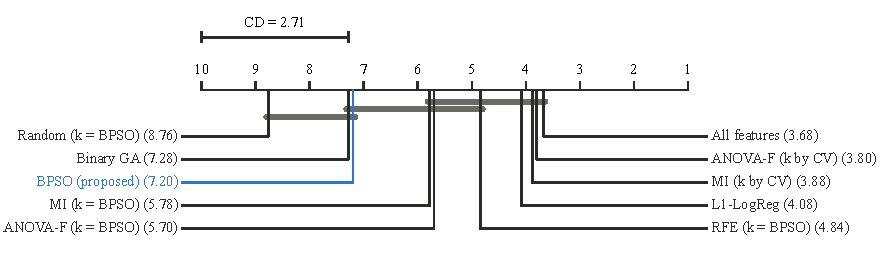
\includegraphics[width=\linewidth]{figures/cd_diagram.pdf}
\caption{Critical-difference diagram of average F1 ranks over 25
dataset--classifier settings. Methods joined by a horizontal bar are not
significantly different (Nemenyi test, $\alpha = 0.05$, CD = 2.71).}
\label{fig:cd}
\end{figure}

Across all five datasets and five classifiers, the Friedman test rejected the
hypothesis that all methods perform equally (Table~\ref{tab:friedman},
Fig.~\ref{fig:cd}). BPSO ranked eighth of ten. It was not significantly
different from the genetic algorithm, RFE, the fixed-size filters or random
subsets, and it was significantly behind all features, both cross-validated
filters and L1-LogReg (rank differences larger than the CD of 2.71). The
methods that keep more features rank highest, which is expected on datasets
with only 8--30 features. Fig.~\ref{fig:boxplot} shows the per-fold
distribution of F1 and ROC-AUC on WDBC.

\begin{figure}[!t]
\centering
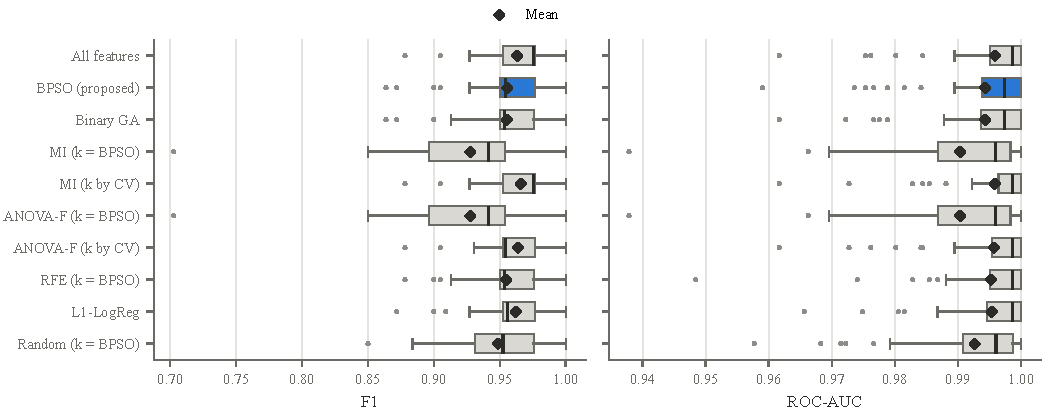
\includegraphics[width=\linewidth]{figures/method_comparison_breast_cancer.pdf}
\caption{F1 and ROC-AUC over 50 outer folds on WDBC (SVM) for all ten
methods; diamonds mark the means.}
\label{fig:boxplot}
\end{figure}

\subsection{Convergence, Stability and Runtime}

BPSO and the genetic algorithm converged to almost the same best fitness, and
most of the improvement happened within the first 15--20 iterations
(Fig.~\ref{fig:convergence}). The mean fitness of the swarm rose again after
about 10 iterations, showing that the swarm kept exploring rather than
collapsing to one solution. Selection stability was moderate: the Jaccard
similarity of BPSO subsets across folds ranged from 0.37 (WDBC) to 0.61 (Pima),
similar to the genetic algorithm (0.34--0.60) and lower than L1-LogReg
(0.67--0.85) and the filters. BPSO took 1.5--8.9\,s per fold, about 1.3--2
times the genetic algorithm and two to three orders of magnitude more than the
filter methods (0.01--0.6\,s).

\begin{figure}[!t]
\centering
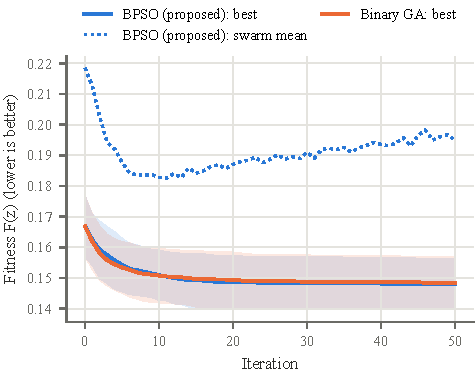
\includegraphics[width=0.9\linewidth]{figures/convergence_heart_cleveland.pdf}
\caption{Best fitness per iteration for BPSO and the genetic algorithm on the
Heart dataset (mean and range over outer folds); the dotted line is the mean
fitness of the BPSO swarm.}
\label{fig:convergence}
\end{figure}

\subsection{Selected Features}

Table~\ref{tab:features} lists the features most often selected by BPSO
across the 50 folds. Several agree with known clinical markers: glucose and
BMI for diabetes (selected in every fold, Fig.~\ref{fig:freq}), specific
gravity and haemoglobin for chronic kidney disease, and the number of major
vessels and thalassemia result for heart disease.

\begin{table}[!t]
\centering
\caption{Most frequently selected features by BPSO (fraction of 50 folds)}
\label{tab:features}
\footnotesize
\setlength{\tabcolsep}{3pt}
\begin{tabular}{lp{0.74\linewidth}}
\toprule
\textbf{Dataset} & \textbf{Features (selection frequency)} \\
\midrule
WDBC & worst smoothness (0.90), worst symmetry (0.84), area error (0.76), worst concavity (0.72), mean texture (0.64) \\
CKD & specific gravity (1.00), haemoglobin (1.00), appetite (0.88), diabetes mellitus (0.88), hypertension (0.84) \\
Heart & major vessels \textit{ca} (1.00), thalassemia (1.00), chest-pain type (0.82), max.\ heart rate (0.76), sex (0.68) \\
ILPD & age (1.00), SGPT (0.86), alkaline phosphatase (0.56), total bilirubin (0.42) \\
Pima & glucose (1.00), BMI (1.00), diabetes pedigree (0.84), insulin (0.62), age (0.54) \\
\bottomrule
\end{tabular}
\end{table}

\begin{figure}[!t]
\centering
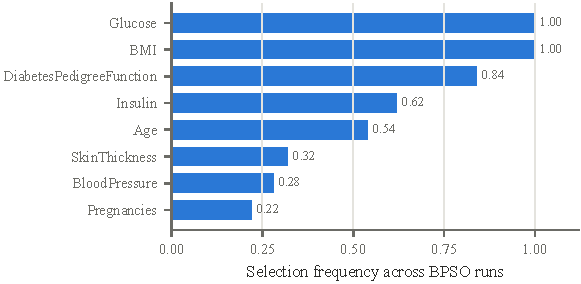
\includegraphics[width=0.9\linewidth]{figures/feature_frequency_pima_diabetes.pdf}
\caption{Selection frequency of each feature by BPSO across 50 outer folds on
the Pima dataset.}
\label{fig:freq}
\end{figure}

\subsection{Sensitivity to $\alpha$}
\label{sec:alpha}

Lowering $\alpha$ puts more weight on subset size (Table~\ref{tab:alpha},
Fig.~\ref{fig:alpha}). On WDBC, $\alpha = 0.90$ kept F1 at 0.953 with about 7
of 30 features (77\,\% reduction), compared with 0.961 and 14 features at
$\alpha = 0.99$. On CKD, $\alpha = 0.95$ kept F1 at 0.995 with about 8 of 24
features. On ILPD a single feature gave the same F1 as four features, but a
much lower ROC-AUC (0.61 vs.\ 0.72), which shows that F1 alone is not
informative on this imbalanced dataset.

\begin{table}[!t]
\centering
\caption{Effect of $\alpha$: mean selected features / F1 (20 runs each)}
\label{tab:alpha}
\footnotesize
\setlength{\tabcolsep}{3pt}
\begin{tabular}{lcccc}
\toprule
\textbf{Dataset (clf.)} & $\boldsymbol{\alpha=0.80}$ & $\boldsymbol{0.90}$ & $\boldsymbol{0.95}$ & $\boldsymbol{0.99}$ \\
\midrule
WDBC (SVM)  & 5.0 / .942 & 6.8 / .953 & 9.9 / .960 & 14.3 / .961 \\
CKD (RF)    & 3.9 / .977 & 6.3 / .987 & 7.7 / .995 & 12.2 / .999 \\
Heart (LR)  & 3.3 / .783 & 4.0 / .790 & 5.0 / .796 & 7.7 / .808 \\
ILPD (LR)   & 1.0 / .832 & 1.4 / .833 & 2.8 / .831 & 4.2 / .832 \\
Pima (LR)   & 1.0 / .574 & 2.1 / .602 & 2.7 / .609 & 4.6 / .616 \\
\bottomrule
\end{tabular}
\end{table}

\begin{figure}[!t]
\centering
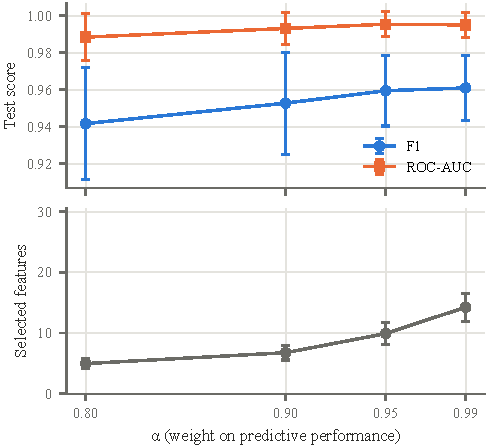
\includegraphics[width=0.85\linewidth]{figures/alpha_sensitivity_breast_cancer.pdf}
\caption{Effect of the trade-off weight $\alpha$ on test F1, ROC-AUC (top) and
number of selected features (bottom) on WDBC (SVM).}
\label{fig:alpha}
\end{figure}

% ---------------------------------------------------------------------------
\section{Discussion}

The results answer the research question in two parts. First, BPSO does
produce substantially smaller models: it removed 38--58\,\% of the features
on every dataset, while the F1-score stayed within about 0.015 of the
all-feature model and the difference in F1 was not statistically significant
on any dataset. For clinical use, where each feature may correspond to a
laboratory test, this reduction can lower data-collection cost and make
models easier to inspect. Second, BPSO did not improve predictive performance.
The selected-feature models performed slightly worse than the full-feature
baselines on most dataset--classifier pairs, with significantly lower ROC-AUC
on three datasets, and simple cross-validated filters ranked higher overall.

Several explanations are consistent with these findings. The datasets are
low-dimensional (8--30 features) and mostly contain informative clinical
variables, so removing features mainly loses information rather than noise.
The fitness function optimises inner accuracy with a logistic-regression
wrapper, while evaluation uses F1 and ROC-AUC with five different classifiers;
this mismatch is a likely reason for the ROC-AUC losses on the imbalanced ILPD
and Pima datasets. Stochastic search variability is also visible: BPSO subsets
changed considerably between folds (Jaccard 0.37--0.61), because several
different subsets reach nearly identical fitness. For interpretation,
selection frequency over many runs (Table~\ref{tab:features}) is therefore
more reliable than any single selected subset. Where BPSO did help---on WDBC,
whose 30 features are strongly correlated---its subsets outperformed
same-size filter subsets, which is consistent with a wrapper choosing
complementary rather than individually strong features. Finally, BPSO and a
genetic algorithm with the same fitness gave practically identical results,
suggesting that the fitness definition matters more than the choice of
metaheuristic, and $\alpha$ is the main control over the size--accuracy
trade-off.

% ---------------------------------------------------------------------------
\section{Limitations and Future Work}

The method's performance depends on the dataset, preprocessing choices,
classifier, fitness function, and stochastic optimization settings. The five
datasets are small, public and low-dimensional; results may differ on
high-dimensional data such as gene expression, where wrapper selection is
usually more beneficial. A reduced search budget (20 particles, 50 iterations)
and 5 repetitions were used. The headline classifier in Table~\ref{tab:main}
was chosen by BPSO's best ROC-AUC, which slightly favours BPSO in that table;
the Friedman analysis over all classifiers does not have this bias. Missing
values were handled by simple median and mode imputation, and no external
validation cohort was used, so the models are not clinically validated.
Future work may optimise ROC-AUC or balanced accuracy in the fitness function,
test V-shaped transfer functions and multi-objective (Pareto) formulations,
add stability or measurement cost to the objective, evaluate high-dimensional
datasets, and validate the workflow with external clinical data.

% ---------------------------------------------------------------------------
\section{Conclusion}

This paper applied Binary Particle Swarm Optimization to feature selection
for disease prediction and evaluated it on five public datasets against nine
alternatives, five classifiers and 50 repeated cross-validation folds per
dataset. Candidate feature subsets are represented as binary particles and
evaluated using a fitness function that balances predictive performance with
subset size. BPSO reduced the number of features by 38--58\,\% with a small,
mostly non-significant loss in F1-score, and selected clinically plausible
features. However, it did not outperform the full feature set or simple
cross-validated filters, and it ranked similarly to a genetic algorithm. On
low-dimensional clinical data, BPSO is therefore best viewed as a tool for
building compact and interpretable models rather than for improving accuracy.

% ---------------------------------------------------------------------------
\begin{thebibliography}{99}

\bibitem{kennedy1995}
J.~Kennedy and R.~Eberhart, ``Particle swarm optimization,'' in \emph{Proc.
IEEE International Conference on Neural Networks}, vol.~4, 1995,
pp. 1942--1948.

\bibitem{kennedy1997}
J.~Kennedy and R.~C. Eberhart, ``A discrete binary version of the particle
swarm algorithm,'' in \emph{Proceedings of the IEEE International Conference
on Systems, Man, and Cybernetics}, 1997, pp. 4104--4108.

\bibitem{pedregosa2011}
F.~Pedregosa \emph{et~al.}, ``Scikit-learn: Machine Learning in Python,''
\emph{Journal of Machine Learning Research}, vol.~12, pp. 2825--2830, 2011.

\bibitem{guyon2003}
I.~Guyon and A.~Elisseeff, ``An introduction to variable and feature
selection,'' \emph{Journal of Machine Learning Research}, vol.~3,
pp. 1157--1182, 2003.

\bibitem{kohavi1997}
R.~Kohavi and G.~H. John, ``Wrappers for feature subset selection,''
\emph{Artificial Intelligence}, vol.~97, no.~1--2, pp. 273--324, 1997.

\bibitem{tibshirani1996}
R.~Tibshirani, ``Regression shrinkage and selection via the lasso,''
\emph{Journal of the Royal Statistical Society: Series B}, vol.~58, no.~1,
pp. 267--288, 1996.

\bibitem{xue2016}
B.~Xue, M.~Zhang, W.~N. Browne, and X.~Yao, ``A survey on evolutionary
computation approaches to feature selection,'' \emph{IEEE Transactions on
Evolutionary Computation}, vol.~20, no.~4, pp. 606--626, 2016.

\bibitem{chuang2008}
L.-Y. Chuang, H.-W. Chang, C.-J. Tu, and C.-H. Yang, ``Improved binary PSO
for feature selection using gene expression data,'' \emph{Computational
Biology and Chemistry}, vol.~32, no.~1, pp. 29--38, 2008.

\bibitem{elbedwehy2012}
M.~N. Elbedwehy, H.~M. Zawbaa, N.~Ghali, and A.~E. Hassanien, ``Detection of
heart disease using binary particle swarm optimization,'' in \emph{Proc.
Federated Conference on Computer Science and Information Systems (FedCSIS)},
2012, pp. 177--182.

\bibitem{pathan2022}
M.~S. Pathan, A.~Nag, M.~M. Pathan, and S.~Dev, ``Analyzing the impact of
feature selection on the accuracy of heart disease prediction,''
\emph{Healthcare Analytics}, vol.~2, art. no. 100060, 2022.

\bibitem{fajri2023}
Y.~A. Z.~A. Fajri, W.~Wiharto, and E.~Suryani, ``Hybrid model feature
selection with the bee swarm optimization method and Q-learning on the
diagnosis of coronary heart disease,'' \emph{Information}, vol.~14, no.~1,
p.~15, 2023, doi: 10.3390/info14010015.

\bibitem{namli2024}
{\"O}.~H. Naml{\i}, S.~Yan{\i}k, A.~Erdo{\u{g}}an, and A.~Schmeink, ``A novel
ensemble artificial intelligence approach for coronary artery disease
prediction,'' \emph{International Journal of Intelligent Computing and
Cybernetics}, vol.~17, no.~3, 2024.

\bibitem{zomorodi2021}
M.~Zomorodi-Moghadam, M.~Abdar, Z.~Davarzani, X.~Zhou, P.~P{\l}awiak, and
U.~R. Acharya, ``Hybrid particle swarm optimization for rule discovery in the
diagnosis of coronary artery disease,'' \emph{Expert Systems}, vol.~38,
art. no. e12485, 2021, doi: 10.1111/exsy.12485.

\bibitem{street1993}
W.~N. Street, W.~H. Wolberg, and O.~L. Mangasarian, ``Nuclear feature
extraction for breast tumor diagnosis,'' in \emph{Proc. SPIE Biomedical Image
Processing and Biomedical Visualization}, vol.~1905, 1993, pp. 861--870.

\bibitem{rubini2015}
L.~Rubini, P.~Soundarapandian, and P.~Eswaran, ``Chronic Kidney Disease,''
UCI Machine Learning Repository, 2015.

\bibitem{janosi1988}
A.~Janosi, W.~Steinbrunn, M.~Pfisterer, and R.~Detrano, ``Heart Disease,''
UCI Machine Learning Repository, 1988, doi: 10.24432/C52P4X.

\bibitem{ramana2012}
B.~Ramana and N.~Venkateswarlu, ``ILPD (Indian Liver Patient Dataset),''
UCI Machine Learning Repository, 2012.

\bibitem{smith1988}
J.~W. Smith, J.~E. Everhart, W.~C. Dickson, W.~C. Knowler, and R.~S.
Johannes, ``Using the ADAP learning algorithm to forecast the onset of
diabetes mellitus,'' in \emph{Proc. Annual Symposium on Computer Applications
in Medical Care}, 1988, pp. 261--265.

\bibitem{detrano1989}
R.~Detrano \emph{et~al.}, ``International application of a new probability
algorithm for the diagnosis of coronary artery disease,'' \emph{The American
Journal of Cardiology}, vol.~64, no.~5, pp. 304--310, 1989, doi:
10.1016/0002-9149(89)90524-9.

\bibitem{shi1998}
Y.~Shi and R.~Eberhart, ``A modified particle swarm optimizer,'' in
\emph{Proc. IEEE International Conference on Evolutionary Computation}, 1998,
pp. 69--73.

\bibitem{guyon2002}
I.~Guyon, J.~Weston, S.~Barnhill, and V.~Vapnik, ``Gene selection for cancer
classification using support vector machines,'' \emph{Machine Learning},
vol.~46, pp. 389--422, 2002.

\bibitem{holm1979}
S.~Holm, ``A simple sequentially rejective multiple test procedure,''
\emph{Scandinavian Journal of Statistics}, vol.~6, no.~2, pp. 65--70, 1979.

\bibitem{demsar2006}
J.~Dem{\v{s}}ar, ``Statistical comparisons of classifiers over multiple data
sets,'' \emph{Journal of Machine Learning Research}, vol.~7, pp. 1--30, 2006.

\end{thebibliography}

\end{document}
